%----------------------------------------------------------------------------------------
%	Capítulo 3
%----------------------------------------------------------------------------------------

\doublespacing
%% NUEVO CAPITULO X
\chapter{Diseño Mecatrónico}

%% NUEVA SECCIÓN X.X
\section{Desarrollo de proyecto conceptual}

El diseño conceptual es parte del proceso de diseño en la que -mediante la identificación de problemas esenciales a través de la abstracción, el establecimiento de estructuras funcionales, búsqueda de principios de funcionamiento adecuados y su combinación en una estructura global- se establece a través de la elaboración de un principio de solución.\cite[p.~159]{Pahl2007}

%% NUEVO SUBSECCION X.X.X
\subsection{Lista de requerimientos}

La lista de requerimientos (Tabla REF) se formuló mediante la realización de entrevistas (Anexo  A1) en las cuales se recopilaron aspectos requerimientos implícitos y explícitos de calidad y cantidad que debe tener el sistema en general. Dicha entrevista se planteó con las recomendaciones que muestra el libro \textit{Engineering Design}\footnote{Engineering Design – A Systematic Approach.\cite[p.~144-158]{Pahl2007}}.

\begin{savenotes}
	% Please add the following required packages to your document preamble:
	% \usepackage{multirow}
	% \usepackage[table,xcdraw]{xcolor}
	% If you use beamer only pass "xcolor=table" option, i.e. \documentclass[xcolor=table]{beamer}
	% \usepackage{longtable}
	% Note: It may be necessary to compile the document several times to get a multi-page table to line up properly
	\scriptsize
	\begin{longtable}{|c|p{0.6cm}|p{10cm}|c|}		
		\caption{Resumen de los requerimientos del sistema.}
		\label{tab:resumen de los requerimientos del sistema}\\
		\hline
		\rowcolor[HTML]{A6A6A6} 
		\multicolumn{4}{|c|}{\cellcolor[HTML]{A6A6A6}{\color[HTML]{000000} \textbf{LISTA DE REQUERIMIENTOS}}} \\ \hline
		\endfirsthead
		%
		\multicolumn{4}{c}%
		{{Tabla \thetable\ continuación de la anterior página.}} \\
		\hline
		\rowcolor[HTML]{A6A6A6} 
		\multicolumn{4}{|c|}{\cellcolor[HTML]{A6A6A6}{\color[HTML]{000000} \textbf{LISTA DE REQUERIMIENTOS}}} \\ \hline
		\rowcolor[HTML]{D9D9D9} 
		\textbf{PROYECTO} &
		\multicolumn{2}{c|}{\cellcolor[HTML]{D9D9D9}\textbf{\begin{tabular}[c]{@{}c@{}}DISEÑO DE CLASIFICADORA Y CONTADORA\\  DE TRUCHAS ARCOÍRIS (Oncorhynchus mykiss)\\ DE 10 A 20 CM. PARA LA CRIANZA DE TRUCHAS\\ EN LA LAGUNA DE PAUCARCOCHA\end{tabular}}} &
		\textbf{\begin{tabular}[c]{@{}c@{}}Fecha:\\ 2020-05-07\\ Página 1 de 1\end{tabular}} \\ \hline
		\rowcolor[HTML]{D9D9D9} 
		{\color[HTML]{000000} \textbf{\begin{tabular}[c]{@{}c@{}}Última \\ modificación\end{tabular}}} &
		{\color[HTML]{000000} \textbf{\begin{tabular}[c]{@{}c@{}}D/\\ E\end{tabular}}} &
		\multicolumn{1}{c|}{\cellcolor[HTML]{D9D9D9}{\color[HTML]{000000} \textbf{Requerimientos}}} &
		{\color[HTML]{000000} \textbf{Reponsable}} \\ \hline
		\endhead
		%
		\rowcolor[HTML]{D9D9D9} 
		\textbf{PROYECTO} &
		\multicolumn{2}{c|}{\cellcolor[HTML]{D9D9D9}\textbf{\begin{tabular}[c]{@{}c@{}}DISEÑO DE CLASIFICADORA Y CONTADORA\\  DE TRUCHAS ARCOÍRIS (Oncorhynchus mykiss)\\ DE 10 A 20 CM. PARA LA CRIANZA DE TRUCHAS\\ EN LA LAGUNA DE PAUCARCOCHA\end{tabular}}} &
		\textbf{\begin{tabular}[c]{@{}c@{}}Fecha:\\ 2020-05-07\\ Página 1 de 1\end{tabular}} \\ \hline
		\rowcolor[HTML]{D9D9D9} 
		{\color[HTML]{000000} \textbf{\begin{tabular}[c]{@{}c@{}}Última \\ modificación\end{tabular}}} &
		{\color[HTML]{000000} \textbf{\begin{tabular}[c]{@{}c@{}}D/E\footnote{Deseo (D) y exigencia (E).}\end{tabular}}} &
		\multicolumn{1}{c|}{\cellcolor[HTML]{D9D9D9}{\color[HTML]{000000} \textbf{Requerimientos}}} &
		{\color[HTML]{000000} \textbf{Reponsable}} \\ \hline
		
		
					&    & \underline{Función principal:}																										& P.D.V. 	\\
		2019-09-24  & E  & Clasificar y contar truchas arcoíris de 10 a 20 $ cm $. en al menos 2 salidas y enviar un reporte de la clasificación y el conteo.   & \multicolumn{1}{l|}{}	\\ 
					&    & \underline{Geometría:}																												& \multicolumn{1}{l|}{}	\\
		2019-09-24  & E  & El sistema no debe exceder los 200x200x200 $ cm $.																					& \multicolumn{1}{l|}{}	\\ 
					&    & \underline{Fuerzas:}																													& \multicolumn{1}{l|}{}	\\
		2019-09-24  & E  & Pesar menos de 200 $ kg $.																											& \multicolumn{1}{l|}{}	\\ 
					&    & \underline{Energía:}																													& \multicolumn{1}{l|}{}	\\
		2019-10-05  & E  & Usará baterías DC.																													& \multicolumn{1}{l|}{}	\\ 	
		2019-09-24  & E  & Funcionar desde -10 a 40 °C.																											& \multicolumn{1}{l|}{}	\\ 	
		2019-09-24  & D  & La máquina debe enviar la información.																								& \multicolumn{1}{l|}{}	\\ 	
					&    & \underline{Materiales:}																												& \multicolumn{1}{l|}{}	\\
		2019-09-22  & E  & La máquina debe ser inoxidable.																										& \multicolumn{1}{l|}{}	\\ 	
		2019-09-20  & E  & La máquina no debe desprender ningún residuo que pueda contaminar el agua.															& \multicolumn{1}{l|}{}	\\ 	
		2019-09-25  & D  & Los materiales de manufactura deben poder ser adquiridos en el mercado peruano.														& \multicolumn{1}{l|}{}	\\ 			
					&    & \underline{Señales:}																													& \multicolumn{1}{l|}{}	\\
		2019-09-24  & E  & Se debe enviar una señal en caso de fallo del sistema y pausar el proceso.															& \multicolumn{1}{l|}{}	\\ 	
					&    & \underline{Hardware:}																												& \multicolumn{1}{l|}{}	\\
		2019-10-05  & E  & La máquina debe usar cámaras o dispositivos similares para obtener imágenes.															& \multicolumn{1}{l|}{}	\\ 		
					&    & \underline{Software:}																												& \multicolumn{1}{l|}{}	\\
		2019-10-05  & D  & El sistema generará un reporte de la clasificación y conteo.																			& \multicolumn{1}{l|}{}	\\ 	
					&    & \underline{Costos:}   																												& \multicolumn{1}{l|}{}	\\ 
		2019-09-24  & D  & El precio unitario menor a 10 mil dólares.       								    												& \multicolumn{1}{l|}{}	\\  \hline
		
		
		\rowcolor[HTML]{D9D9D9} 
		\multicolumn{1}{|l|}{\cellcolor[HTML]{D9D9D9}{\color[HTML]{000000} }} &
		\multicolumn{2}{c|}{\cellcolor[HTML]{D9D9D9}{\color[HTML]{000000} \textbf{Última modificación: 2019-10-05}}} &
		{\color[HTML]{000000} } \\ \hline
	\end{longtable}

\end{savenotes}

%% NUEVO SUBSECCION X.X.X
\subsection{Caja negra}

La caja negra mostrada en la Figura \ref{fig:caja negra del sistema} representa la energía (flecha continua), materia (flecha gruesa) y señales (flecha discontinua) que necesita y brinda el sistema para funcionar como un sistema clasificador y contador de truchas de un determinado rango según la lista de requerimientos mostrada en la Tabla REF.

\begin{figure}[H]
	\centering
	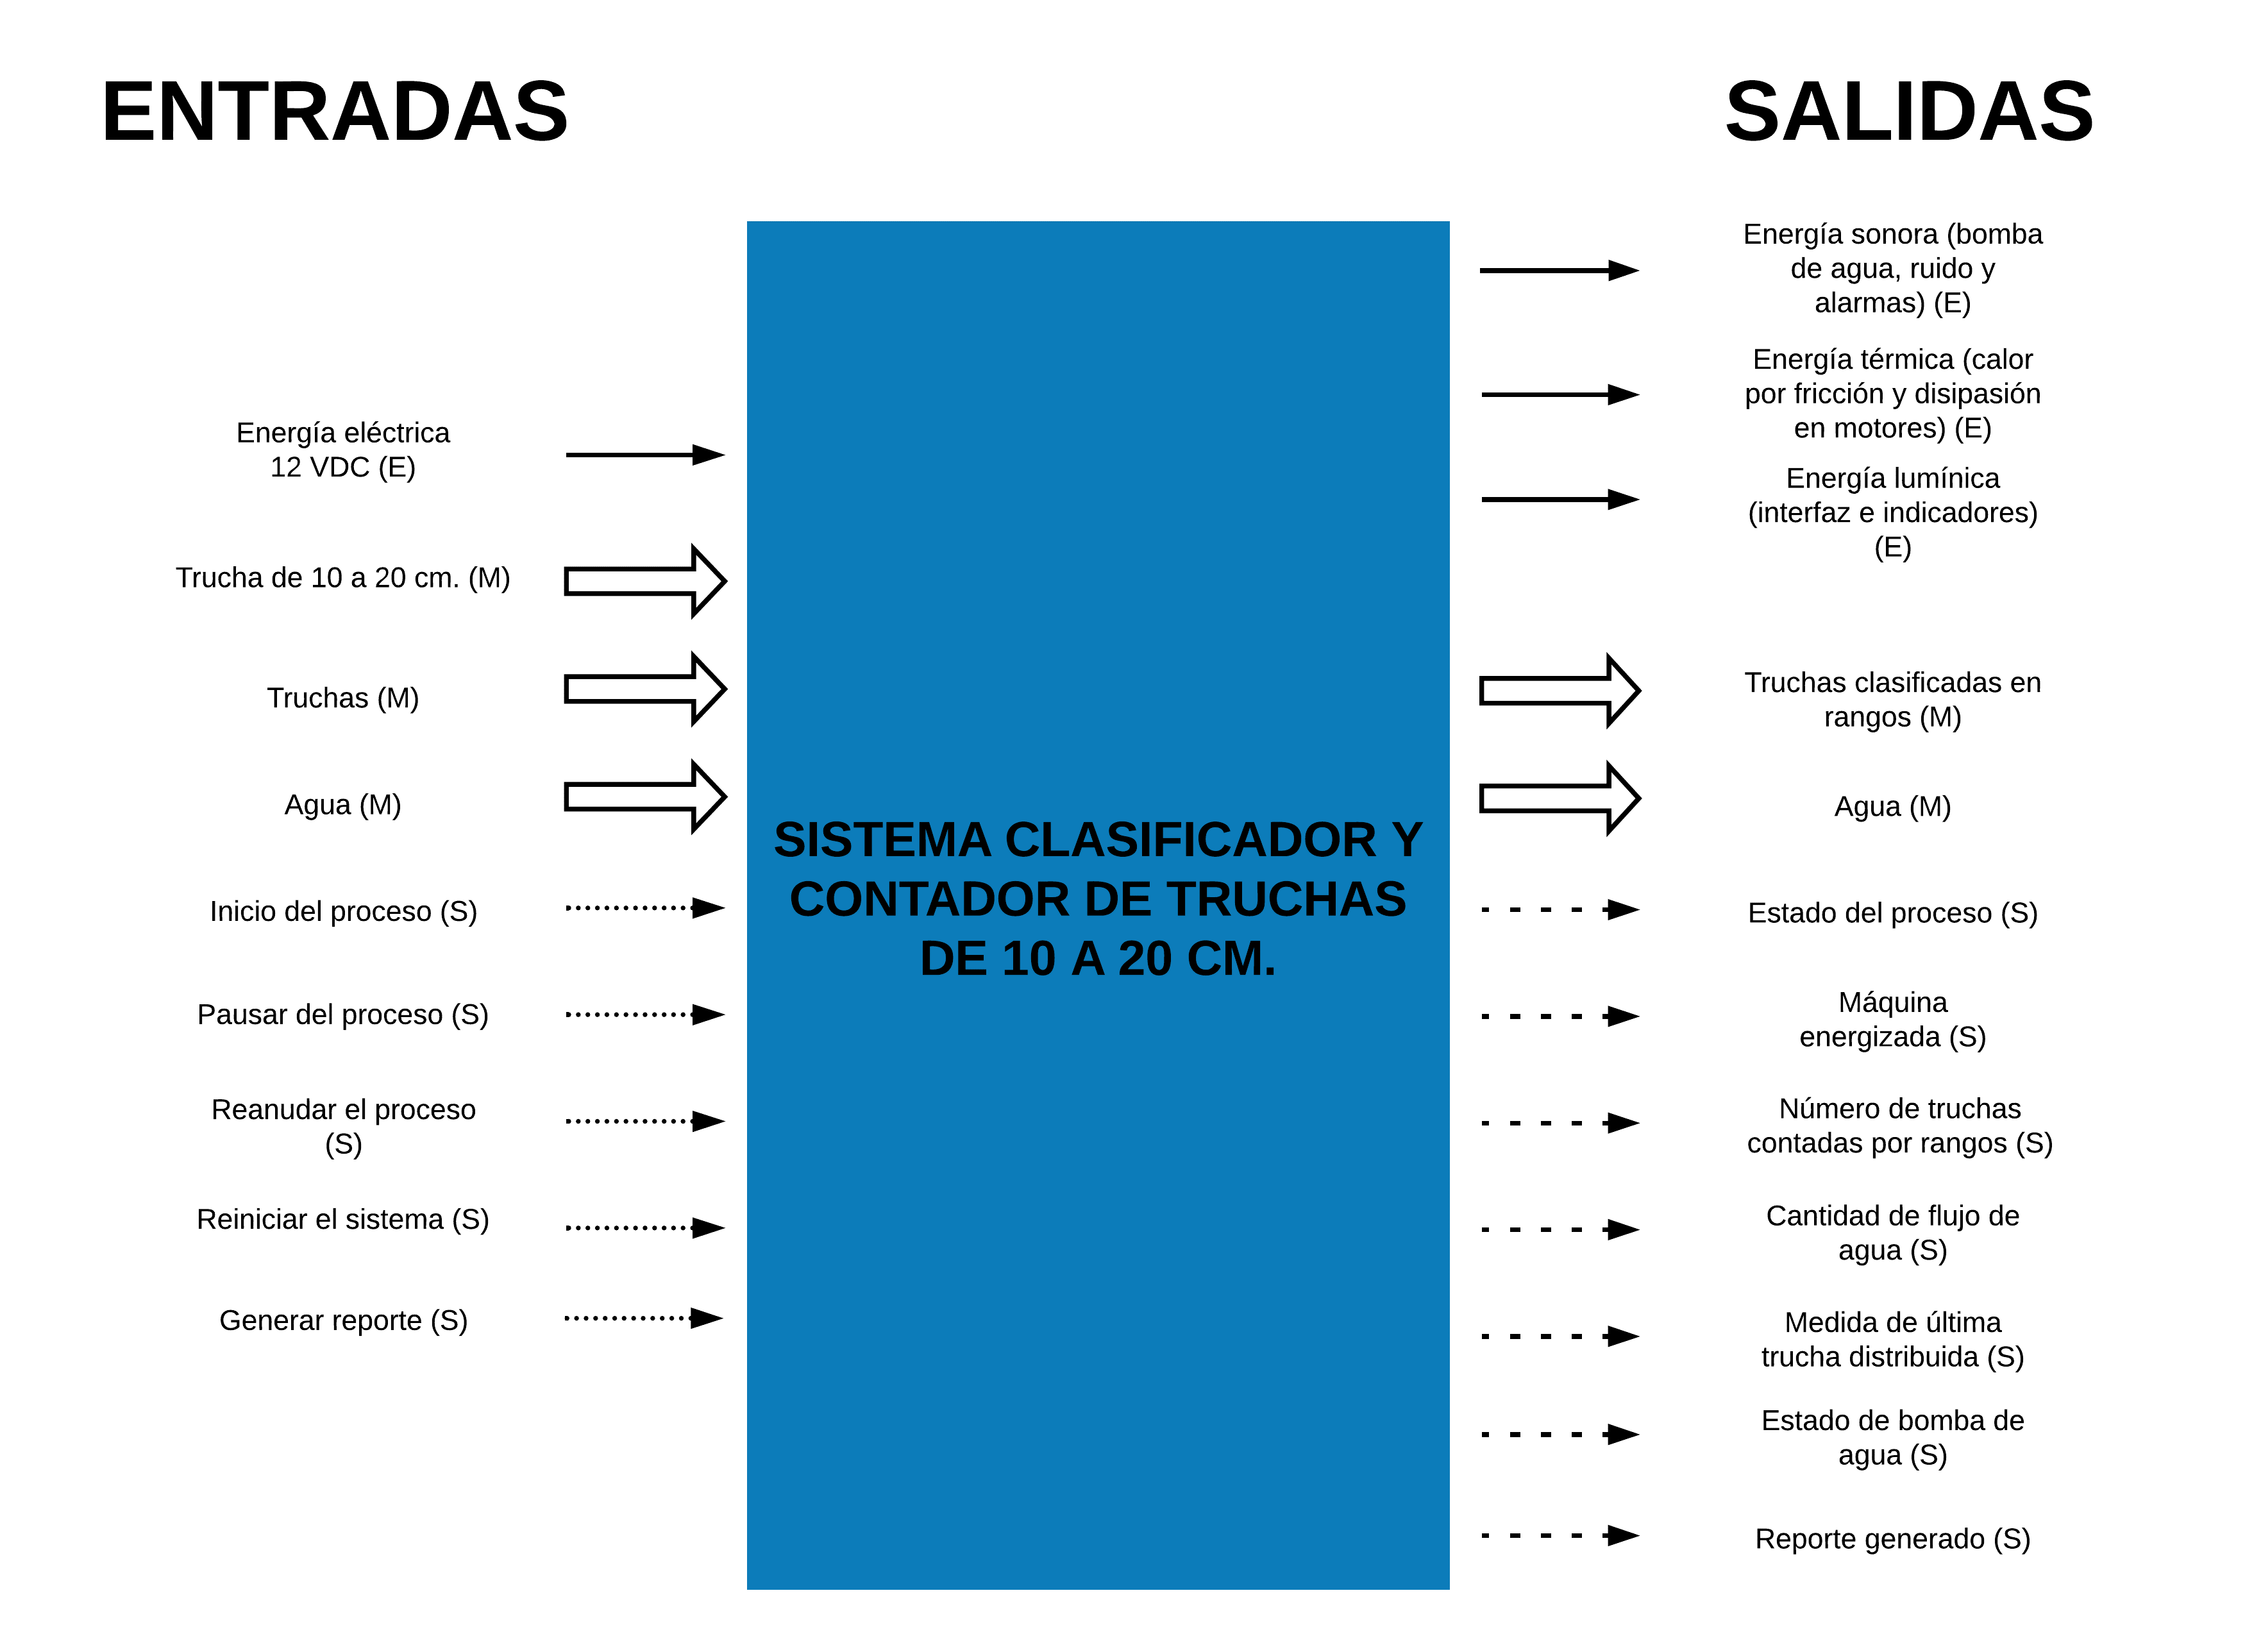
\includegraphics[width=1\textwidth]{chapter3/caja negra del sistema.png}
	\caption{Caja negra del sistema.}
	Fuente: Elaboración propia.
	\label{fig:caja negra del sistema}
\end{figure}

%% NUEVA SUB-SUB-SECCION X.X.X.X
\subsubsection{Función principal}

El sistema tiene como función principal clasificar truchas que provienen de un estanque o jaula flotante que tiene truchas que necesitan ser redistribuidas según sus dimensiones.

%% NUEVA SUB-SUB-SECCION X.X.X.X
\subsubsection{Entradas}

El sistema tiene entradas de diversos tipos: energía, materia y señal. La entrada de energía es únicamente una batería de 12 VDC ya que es portable; Las entradas de materia son indispensablemente el agua y las truchas a clasificar; Las señales de entrada para este proceso son las básicas para cualquier proceso de este tipo (\textit{iniciar, pausar, reanudar y reiniciar}), además la señal de generar un reporte para ser analizado y mantener control sobre el cultivo.

%% NUEVA SUB-SUB-SECCION X.X.X.X
\subsubsection{Salidas}

De manera similar a las entradas, las salidas se dividen en energía, materia y señal: El sistema genera tres tipos de energía debido a los actuadores, ruido, alarmas, interfaz e indicadores; Las truchas divididas en hasta tres rangos salen de manera separada; Se muestra el estado del proceso, estado del sistema, número de truchas contadas dependiendo del rango, medida de la última trucha distribuida, estado de la bomba de agua y la señal de reporte generado.

%% NUEVO SUBSECCION X.X.X
\subsection{Estructura de funciones}

Una vez que se ha formulado la caja negra es posible indicar, con el uso de diagrama de bloques, expresar la relación entre entradas y salidas con una solución neutral. Esta relación debe tener la mayor precisión posible. La estructura de funciones global puede desglosarse en sistemas que a su vez se subdividen en funciones.\cite[p.~169-181]{Pahl2007}

%% NUEVA SUB-SUB-SECCION X.X.X.X
\subsubsection{Lista de funciones por subsistema}

%% NUEVO SUBSECCION X.X.X
\subsection{Matriz morfológica}

%% NUEVO SUBSECCION X.X.X
\subsection{Conceptos de solución}

%% NUEVA SUB-SUB-SECCION X.X.X.X
\subsubsection{Concepto de solución N° 1}

%% NUEVA SUB-SUB-SECCION X.X.X.X
\subsubsection{Concepto de solución N° 2}

%% NUEVA SUB-SUB-SECCION X.X.X.X
\subsubsection{Concepto de solución N° 3}

%% NUEVO SUBSECCION X.X.X
\subsection{Evaluación técnico-económica}

%% NUEVA SUB-SUB-SECCION X.X.X.X
\subsubsection{Criterios técnicos}

%% NUEVA SUB-SUB-SECCION X.X.X.X
\subsubsection{Criterios económicos}

%% NUEVA SUB-SUB-SECCION X.X.X.X
\subsubsection{Elección de concepto óptimo}

%% NUEVO SUBSECCION X.X.X
\subsection{Diagrama de operaciones de solución escogida}

%%%%%%% FALTA PUNTOS 
%%%%%%% FALTA PUNTOS 
%%%%%%% FALTA PUNTOS 
%%%%%%% FALTA PUNTOS 
%%%%%%% FALTA PUNTOS 
%%%%%%% FALTA PUNTOS 
%%%%%%% FALTA PUNTOS 
%%%%%%% FALTA PUNTOS 



